\documentclass{standalone}
\usepackage{tikz}

\begin{document}

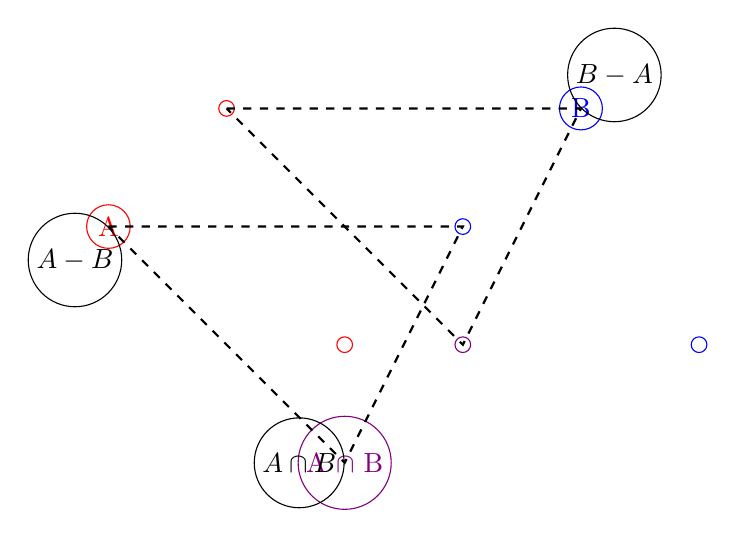
\begin{tikzpicture}[scale=1.5, every node/.style={circle, draw, inner sep=2pt}]

    % Define coordinates for the points
    \coordinate (A1) at (-2, 2);
    \coordinate (A2) at (-1, 3);
    \coordinate (A3) at (0, 1);
    
    \coordinate (B1) at (1, 2);
    \coordinate (B2) at (2, 3);
    \coordinate (B3) at (3, 1);
    
    \coordinate (C1) at (0, 0);
    \coordinate (C2) at (1, 1);

    % Draw the sets A, B, and C
    \node[red] at (A1) {A};
    \node[red] at (A2) {};
    \node[red] at (A3) {};

    \node[blue] at (B1) {};
    \node[blue] at (B2) {B};
    \node[blue] at (B3) {};

    \node[violet] at (C1) {A $\cap$ B};
    \node[violet] at (C2) {};

    % Draw the semi-coarse space X
    \draw[dashed, thick] (A1) -- (B1) -- (C1) -- cycle;
    \draw[dashed, thick] (A2) -- (B2) -- (C2) -- cycle;

    % Add labels
    \node[below left] at (A1) {$A - B$};
    \node[above right] at (B2) {$B - A$};
    \node[left] at (C1) {$A \cap B$};

\end{tikzpicture}

\end{document}